\chapter{Bernoulli and Poisson Processes}
A stochastic process is a mathematical model of a probabilistic experiment that evolves in time and generates a sequence of numerical values. For example, the sequence of daily prices of a stock.

Each numerical value in the sequence is modeled by a random variable, so a stochastic process  is simply a  (finite or  infinite) sequence of random variables. We are still dealing with a single basic experiment that involves outcomes governed by a probability law, and random variables that inherit their probabilistic properties from that law.

However, stochastic processes involve some change in emphasis over our earlier models, such as:
\begin{enumerate}
    \item We tend to focus on the \textit{dependencies} in the sequence of values generated by  the process. For example, how do  future  prices of a stock depend on past values?
    \item We  are often interested in \textit{long-term averages} involving the entire sequence of generated values. For example, what is the fraction of time that a machine is idle?
    \item We  sometimes wish to characterize the \textit{likelihood} or frequency of certain boundary events. What is the frequency with which some buffer in a computer net­work overflows with data?
\end{enumerate}
There is a wide variety of stochastic processes, but in this book we will only discuss two major categories
\begin{enumerate}
    \item [Arrival] The processes in which occurrences have a characteristic of "arrival". We  will focus on models in which the interarrival times (the times between successive arrivals) are independent \rv. We consider discrete time arrivals and interarrivals (Bernoulli processes) and continuous arrivals and exponentially distributed interarrivals (Poisson process).
    \item [Markov] Experiments that evolve in time and in which the future evolution exhibits a probabilistic dependence on the past. However, we assume a very special type of dependence: the next value depends on past values only through the current value.
\end{enumerate}

\section{Bernoulli Process}
Bernoulli Process can be visualized as a sequence of independent coin tosses where each toss has a fixed probability $p$ which is independent of other trails.

Formally, Bernoulli process is a sequence of \textbf{independent} Bernoulli \RV $X_1,X_2,\ldots$ with
\[
    \Pr(X_i) = \begin{cases}
        \Pr(\text{success at the ith trial)} &= p \\
        \Pr(\text{failure at the ith trial)} &= 1-p
    \end{cases}
\]

Some \rv associated with the Bernoulli Process and their properties
\begin{enumerate}
    \item The binomial with parameters $p$ and $n$. This is the number $S$ of successes in $n$ independent trials. Its PMF, mean, and variance are
    \begin{align*}
        p_S(k) &= \binom{n}{k}p^k(1-p)^{n-k}, \quad k = 0,1,\ldots,n \\
        \E[S] &= np \\
        \var(S)&=np(1-p)
    \end{align*}
    \item The geometric with parameter $p$. This is the number $T$ of trials up to (and including) the first success. Its PMF, mean, and variance are
    \begin{align*}
        p_T(t) &= (1-p)^{t-1}p, \quad t=1,2,\ldots\\
        \E[T]&=1/p\\
        \var(T)&=\frac{1-p}{p^2}
    \end{align*}
\end{enumerate}

\subsection{Independence and Memorylessness}
The independence assumption underlying the Bernoulli process has important implications, including a memorylessness property.
\begin{definition}[Memorylessness]
    Whatever has happened in past trials provides no information on the outcomes of future trials.
\end{definition}

We develop some intuition as this property leads to quick and simple solutions to difficult problems. 
\begin{itemize}
    \item [independence] Let us start by considering random variables that are defined in terms of what happened in a certain set of trials. Consider two \rv $Y=(X_1+X_3)X_6X_7$ and $Z=X_2(X_4+X_5)$ are independent because of no common element. This is generalization of fact that functions of independent \rv are independent.
    \item [fresh start] Suppose now that the Bernoulli process has been running for $n$ time steps with observed values as $X_1,\ldots,X_n$. The sequence of future trials $X_{n+1},X_{n+2},\ldots$ are independent Bernoulli trials and therefore a Bernoulli process. Starting from any given point in time, the future is also modeled by a Bernoulli process, which is independent of the past.
    \item [first success] The time until first success is a geometric \rv and so failing first $n$ trials provides us with no information about the probability of first success. Due to fresh-start the \rv for the first success after $n$ trials remains unchanged.
    \[
        \Pr(T-n=t|T>n)=(1-p)^{t-1}p=\Pr(T=t), \quad t=1,2,\ldots
    \]
\end{itemize}

\subsection{Interarrival times}
Consider $T_i$ to to be the interarrival time between the $i-1^{th}$ and $i^{th}$ arrival. Since Bernoulli processes have a fresh-start property, $T_i$'s are independent of each other as the time beginning after the $(i-1)^{th}$ arrival tells us nothing about the future. This gives us an alternate definition of the Bernoulli process.

\begin{definition}[Bernoulli Process]
    Start with a sequence of geometric independent \rv $T_1, T_2,\ldots$ with same parameter $p$ and let these be interarrival times. Record a success at time $T_1, T_1+T_2, T_1+T_2+T_3, \ldots$
\end{definition}

\begin{example}
    It has been observed that after a rainy day. the  number of days until it rains again is geometrically distributed with parameter $p$. independent of the past. Find the probability that it rains on both the 5th and the 8th day of the month.

    If we consider the independence of the trails then the answer is $p^2$. \qed
\end{example}

\subsection{$k^{th}$ Arrival time}

The time of the $k^{th}$ arrival $Y_k=T_1+\cdots+T_k$, where $T_i$'s are geometric \rv has
\begin{align}
    \E[Y_k]&=\E[T_1]+\cdots+\E[T_k]=k/p\\
    \var(Y_k)&=\var(T_1)+\cdots+\var(T_k)=\frac{k(1-p)}{p^2}\\
    \label{pascal_pmf}
    p_{Y_k}&=\binom{t-1}{k-1}p^k(1-p)^{t-k}, \quad t=k,k+1,\ldots,
\end{align}
where \ref{pascal_pmf} is known as Pascal PMF of order $k$.

\subsection{Splitting and merging of Bernoulli process}
Consider a Bernoulli process of arrivals with probability of each arrival as $p$ independent of other arrivals. Suppose that with probability $q$ we either keep it or with probability $1-q$ we discard it. The probability of keeping the arrival is now $pq$ and this it is also a Bernoulli process with probability $pq$. Similarly the discarded arrivals also constitute a Bernoulli process with probability $p(1-q)$.

\begin{remark}
    To prove that a process is Bernoulli we need that the probability of each arrival must be same for every arrival and is independent from other arrivals. The arrivals were independent before splitting and thus remains independent after splitting.
\end{remark}

Similarly in case of merging, if the probabilities of the processes are $p$ and $q$ respectively, then the merged process will be a Bernoulli process with probability $(1-p)(1-q)$ or $p+q-pq$.

\subsection{The Poisson approximation to the Binomial}
The number of successes in $n$ independent Bernoulli trails is a Bernoulli \rv with parameters $n$ and $p$ with mean as $np$. If we let $n$ grow large and simultaneously decrease $p$ to keep the mean constant, we can approximate Poisson process as Bernoulli process with large trails and small probability of each success.

\begin{enumerate}
    \item The poisson \rv $Z$ with parameter $\lambda$ takes nonnegative integer values described by the PMF 
    \[p_Z(k)=e^{-\lambda}\frac{\lambda^k}{k!}, \quad k=0,1,\ldots,\]
    The mean and variance are $\E[Z]=\var(Z)=\lambda$.
    \item The binomial probability \[p_S(k)=\binom{n}{k}p^k(1-p)^{n-k}\] converges to $p_Z(k)$ as $n \to \infty$ and $p=\lambda/n$, while keeping $\lambda$ constant.
\end{enumerate}

\section{Poisson process}
The Poisson process is a continuous-time analog of the Bernoulli process and applies to situations where there is no natural way of dividing time into discrete periods.

\begin{example}[Traffic Accidents]
    Suppose that to model traffic accidents we keep a 1-minute interval and mark a "success" if any accidents happen in that interval. This can be a bernoulli process as the time slots are independent with same probability.
    
    It is possible to have two or more accidents happening at the same time but Bernoulli process does not track the exact number of accidents. To get around this, we can choose a smaller time interval but what would it be? a second? a millisecond? Instead, we use the limiting case and arrive at continuous time model. \qed
\end{example}

For an arrival process that evolves in continuous-time, we define
\[P(k,\tau)=P(\text{exactly } k \text{ arrivals happen during interval of length } \tau)\]

We also assume that the probability is same for all intervals of same length $\tau$. We also introduce an arrival rate or intensity of the process as $\lambda$.

\begin{definition}[Poisson process]
    An arrival process is called a Poisson Process with rate $\lambda$ if it satisfies
    \begin{enumerate}
        \item [time-homogeneity] $P(k,\tau)$ of $k$ arrivals is the same for all intervals of length $\tau$.
        
        \textit{All arrivals are equally likely at all times. Analogous to Bernoulli Bernoulli processes having same success probability of each interval as $p$.}

        \item [independence] The number of arrivals during a period is independent of the history of arrivals outside this interval.

        \textit{Analogous to Bernoulli trails being independent of each other.}

        \item [small-interval] The probabilities $P(k,\tau)$ satisfy
        \begin{align*}
            P(0,\tau) &= 1-\lambda\tau+o(\tau)\\
            P(1,\tau) &= \lambda\tau+o_1(\tau)\\
            P(k,\tau) &= o_k(\tau), \quad k=2,3,\ldots
        \end{align*}
        where $o(\tau)$ and $o_k(\tau)$ are asymptotic notations satisfying $\lim_{\tau \to 0}\frac{o_k(\tau)}{\tau}=0$.

        \textit{There can be atmost one arrival with probability $\lambda\tau$ in a small interval $\tau$.}
    \end{enumerate}
\end{definition}

\subsection{Number of Arrivals in an Interval}
Consider a time interval of length $\tau$ and partition it into $\tau/\delta$ periods of small length $\delta$. The probability of two occurrence can be neglected (by \textit{small-interval} property). Different slots are independent (by \textit{independence} property).

Therefore, the probability $P(k, \tau)$ is same as binomial probability of $k$ success in $n=\tau/\delta$ Bernoulli trials with $p=\lambda\delta$.

If $\delta \to 0$, then according to previous section, binomial PMF converges to Poisson PMF with parameter $\lambda\tau$.

\[\boxed{P(k, \tau)=e^{-\lambda\tau}\frac{(\lambda\tau)^k}{k!}, \quad k=0,1,\ldots}\]

\begin{remark}
    The small interval property can be proved by taylor series expansion of above formula.
\end{remark}

The probability law for the first arrival is
\[F_T(t)=\Pr(T\le t)=1-\Pr(T>t)=1-P(0,t)=1-e^{-\lambda t}, \quad t\ge 0\]
Differentiating the CDF $F_T(t)$, we obtain
\[\boxed{f_T(t)=\lambda e^{-\lambda t}, \quad t\ge 0}\]

\subsection{Independence and Memorylessness}
The Poisson process has properties such as
\begin{itemize}
    \item independence of non-overlapping time sets --- For any given time $t>0$, the history of the process after time $t$ is also a Poisson process, and is independent from the history of the process until time $t$.
    \[\Pr(\bar T-t>s)=\Pr(0 \text{ arrivals during }[t,t+s])=P(0,s)=e^{-\lambda s}\]
    \item memorylessness of interarrival time distribution --- Let $t$ be a given time and let $\bar T$ be the time of first arrival after $t$. Then $\bar T -t$ has an exponential distribution with parameter $\lambda$ and is independent of ths history of the process until time $t$.
\end{itemize}
Because Poisson process can be viewed as a limiting case of Bernoulli, therefore it inherits the properties.

\begin{example}[Independence]
    You go to a bank and see all three tellers are busy serving customers and its your turn next. Assuming each customer's service time is identically distributed exponential \rv, what is the probability that you'll be the last one to leave?

    1/3. The time when you'll start serviced, the PDF of the other customers is same as yours because of memorylessness.
\end{example}

\begin{definition}[Poisson Process (Alternative)]
    Start with a sequence of independent \rv $T_1, T_2,\ldots,$ with common parameter $\lambda$ and let these be interarrival times. Record an arrival at $T_1, T_1+T_2, T_1+T_2+T_3,\ldots$, etc.
\end{definition}

\subsection{The $k$th Arrival Time}
The time $Y_k$ of $k$th arrival is equal to $T_1+T_2+\cdots+T_k$ of $k$ independent identically distributed \rv with 
\begin{itemize}
    \item mean and variance as
    \[\E[Y_k]=\E[T_1]+\cdots+\E[T_k]= k/\lambda\]
    \[ \var(Y_k)=\var(T_1)+\cdots+\var(T_k)=k/\lambda^2\]
    \item The PDF of $Y_k$ is given by
    \[f_{Y_k}(y)=\frac{\lambda^ky^{k-1}e^{-\lambda y}}{(k-1)!}, \quad y\ge 0\]
    and is known is Erlang PDF of order $k$.
\end{itemize}

\begin{remark}
    For a small $\delta$, $\delta f_{Y_k}(y)$ gives the probability of $k^{th}$ arrival in the interval $[y,y+\delta]$, i.e. $y\le Y_k \le y+\delta$.
\end{remark}

\subsection{Splitting and Merging of Poisson Process}
Similar to Bernoulli process, 
\begin{enumerate}
    \item [split] An arrival in Poisson process can be kept with probability $p$ and this the splitting is a Poisson process with arrival rate $\lambda p$.
    \item [merge] Two Poisson process with arrival rates as $\lambda_1$ and $\lambda_2$ when merged results in a Poisson Process with rate $\lambda_1 + \lambda_2$. An arrival in merged process has probability $\lambda_1/(\lambda_1+\lambda_2)$ of originating from the first process.
\end{enumerate}
\begin{remark}
    Processes obtain by splitting a Poisson process are independent.
\end{remark}

\subsection{Random Incidence Paradox}

\begin{center}
\tikzset{every picture/.style={line width=0.75pt}} %set default line width to 0.75pt
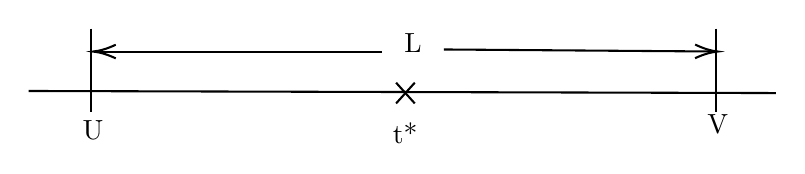
\begin{tikzpicture}[x=0.75pt,y=0.75pt,yscale=-1,xscale=1]
%uncomment if require: \path (0,300); %set diagram left start at 0, and has height of 300

\draw    (119.5,120) -- (479.5,121) ;
\draw    (149.5,90) -- (149.5,130) ;
\draw    (450.5,90) -- (450.5,130) ;
\draw    (305.5,116) -- (296.5,126) ;
\draw    (319.5,100) -- (449.5,100.98) ;
\draw [shift={(451.5,101)}, rotate = 180.43] [color={rgb, 255:red, 0; green, 0; blue, 0 }  ][line width=0.75]    (10.93,-3.29) .. controls (6.95,-1.4) and (3.31,-0.3) .. (0,0) .. controls (3.31,0.3) and (6.95,1.4) .. (10.93,3.29)   ;
\draw    (289.5,101) -- (152.5,101) ;
\draw [shift={(150.5,101)}, rotate = 360] [color={rgb, 255:red, 0; green, 0; blue, 0 }  ][line width=0.75]    (10.93,-3.29) .. controls (6.95,-1.4) and (3.31,-0.3) .. (0,0) .. controls (3.31,0.3) and (6.95,1.4) .. (10.93,3.29)   ;
\draw    (305.5,126) -- (296.5,116) ;

\draw (299,91) node [anchor=north west][inner sep=0.75pt]  [font=\normalsize] [align=left] {L};
\draw (293.5,134) node [anchor=north west][inner sep=0.75pt]   [align=left] {t*};
\draw (144,133) node [anchor=north west][inner sep=0.75pt]   [align=left] {U};
\draw (445,130) node [anchor=north west][inner sep=0.75pt]   [align=left] {V};
\end{tikzpicture}
\end{center}
For a fixed time instant $t^*$, the corresponding interval $[U,V]$ consists of elapsed time $t^* - U$ and remaining time $V-t^*$. These two times are independent and are exponentially distributed with parameter $\lambda$, so the PDF of their sum is Erlang of order two.

This misconception arises an observer is more likely to fall into larger intervals than smaller intervals. Thus the expected length observed is larger than actual expected length.

\begin{example}[Random Incidence on a Non-Poisson Arrival Process]
    Imagine a bus station at which buses arrive with interarrival time alternating between 5 and 55 mins. The average interarrival time is therefore 30 mins. A person shows up at the bus station with all time points in an hour being equally likely.
    The probability of falling in 5 min interval is 1/12 and in 55 min interval is 11/12.
    \[\text{(Expected interarrival time)} \quad 5 \cdot \frac{1}{12} + 55 \cdot \frac{11}{12}=50.83 \gg 30\]
\end{example}

\begin{example}[Questioning a rider from an empty bus]
    Consider the task of calculating percent utilization of buses in a city. There are two approaches
    \begin{enumerate}
        \item Choose a random set of buses and calculate the average riders in it.
        \item Pick random people and ask the number of people that were there in the bus.
    \end{enumerate}
    The second approach is biased upwards because it is more likely for a person to be from a bus with large riders than from nearly empty bus. Empty buses will not be taken into account as there will not be any rider that can account for it.
\end{example}

\section{Sums of \RV}
Let $N,X_1,X_2,\ldots$ be independent \rv and $N$ takes non-negative integer values. Let $Y=X_1+\cdots+X_N$ for positive values of $N$ and $Y=0$ for $N=0$.

\begin{center} \begin{tabu}{|c|c|c|}
    \hline $X_i$ & $N$ & $Y$ \\ \hline
    Bernoulli ($p$) & Binomial ($m, q$) & Binomial ($m, pq$) \\
    Bernoulli ($p$) & Poisson ($\lambda$) & Poisson ($\lambda p$) \\
    Geometric ($p$) & Geometric ($q$) & Geometric ($pq$) \\
    Exponential ($\lambda$) & Geometric ($q$) & Exponential ($\lambda q$)\\
    \hline
\end{tabu} \end{center}

\subsection{Sum of large number of independent arrival process}
The sum of a large number of (not necessarily Poisson) independent arrival processes, can be approximated by a  Poisson process with arrival  rate equal to the sum of the individual arrival  rates. The component processes must have a small rate relative to the total (so that none of them imposes its probabilistic character on the total arrival process) and they must also satisfy some technical mathematical assumptions. Therefore, this property leads to abundance of Poisson-like processes in practice.

For example, the telephone traffic originating in  a city consists of many components, reflecting the phone calls placed by a resident, can be modelled by a Poisson process. Need not be Poisson because some makes calls in batches and usually cannot initiate a second call while on the first call. For the same reasons, auto accidents in a city, customer arrivals at a store, etc tend to be Poisson-like.